\chapter{Transformadors de Mesura i Protecci\'{o}}
\index{transformadors de mesura i protecci\'{o}}

Es tracten en aquest cap\'{\i}tol temes referents als transformadors de
mesura i de protecci\'{o}, tant de tensi\'{o} com d'intensitat. Aquest
tractament es fa des del punt de vista de les normes \textsf{CEI}.
En l'apartat final, es descriuen les normes \textsf{ANSI}, i la seva
correspond\`{e}ncia amb les \textsf{\textsf{CEI}}.

\section{Introducci\'{o}}\index{transformadors de mesura i protecci\'{o}!connexionat}

En la Figura \vref{pic:TT_TI} es representen uns connexionats
habituals d'un transformador de tensi\'{o} (anomenats usualment TT) , a
la part superior, i d'un transformador d'intensitat (anomenats
usualment TI o TC) , a la part inferior. Els sentits de les tensions
i corrents s'han representat tenint en compte els terminals
equivalents (marcats amb un punt) dels primaris i secundaris.
\index{TT}\index{TI}\index{TC}

\begin{figure}[h!]
\hfill
\begin{minipage}[b]{85mm}
\hspace{1.5cm}
    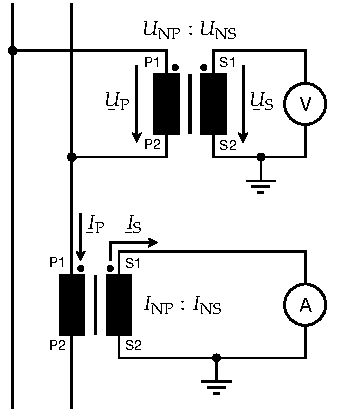
\includegraphics{Imatges/Cap-TrafosMesProt-TI-TT.pdf}
\caption{Transformadors de tensi\'{o} i d'intensitat} \label{pic:TT_TI}
\end{minipage}
\hfill
\begin{minipage}[b][70mm][t]{50mm}
   \begin{align}
      \cmplx{U}\ped{S} &= \cmplx{U}\ped{P} \frac{U\ped{NS}}{U\ped{NP}}
      \\[24mm]
      \cmplx{I}\ped{S} &= \cmplx{I}\ped{P} \frac{I\ped{NS}}{I\ped{NP}}
   \end{align}
\end{minipage}
\end{figure}

Les relacions de transformaci\'{o} nominals d'aquests transformadors de
tensi\'{o} i d'intensitat, s\'{o}n $U\ped{NP}:U\ped{NS}$ i
$I\ped{NP}:I\ped{NS}$ respectivament. Al costat de la Figura
\vref{pic:TT_TI} es poden veure les relacions que lliguen les
tensions i corrents de primari amb les de secundari, suposant que
els transformadors s\'{o}n ideals.

Els terminals del primari es designen \textsf{P1} i \textsf{P2}, i
els del secundari \textsf{S1} i \textsf{S2}; \textsf{P1} i
\textsf{S1} s\'{o}n sempre terminals equivalents.\index{transformadors
de mesura i protecci\'{o}!terminals
equivalents}\index{P1}\index{P2}\index{S1}\index{S2}

Els transformadors de tensi\'{o} es connecten a la l\'{\i}nia principal, en
derivaci\'{o}; el  primari est\`{a} sotm\`{e}s, per tant, a la tensi\'{o} de la
l\'{\i}nia. Els TT per a connexi\'{o} entre fases tenen els dos borns
primaris a\"{\i}llats, mentre que els que estan previstos per ser
connectats entre fase y terra, nom\'{e}s en tenen un d'a\"{\i}llat , ja que
l'altre es connecta directament a terra. Els transformadors de
corrent, en canvi, es connecten amb el primari intercalat en la
l\'{\i}nia principal;  pel primari del TI circula, per tant, la
intensitat de la l\'{\i}nia.

 Com a mesura de protecci\'{o} per a les persones, \'{e}s usual
connectar a terra un dels dos terminals del secundari dels
transformadors. Cal recordar a m\'{e}s, en el cas dels transformadors de
corrent, que el secundari no ha de quedar mai en circuit obert, ja
que es produirien sobretensions que podrien malmetre el
transformador.

\section{Errors de mesura dels transformadors reals}

At\`{e}s que en realitat, els transformadors que es construeixen no s\'{o}n
ideals, tots tenen un error en la transformaci\'{o} de la magnitud
prim\`{a}ria en la secund\`{a}ria, tant pel que fa al m\`{o}dul, com pel que fa
a l'angle.

\subsection{Error de relaci\'{o}}\index{transformadors
de mesura i protecci\'{o}!error de relaci\'{o}}

Aquest \'{e}s l'error de m\`{o}dul existent entre les magnituds prim\`{a}ria i
secundaria; es denomina m\'{e}s espec\'{\i}ficament, error d'intensitat en el
cas dels TI, i error de tensi\'{o} en el cas dels TT.

En el cas dels TI, si $I\ped{P}$ i $I\ped{S}$ s\'{o}n els corrents que
realment circulen pel primari i pel secundari respectivament,
l'error d'intensitat $\epsilon\ped{I}$ val:
\begin{equation}
    \epsilon\ped{I} = \frac{\frac{I\ped{NP}}{I\ped{NS}} I\ped{S} - I\ped{P}} {I\ped{P}}
\end{equation}
\index{$\epsilon\ped{I}$}

En el cas dels TT, si $U\ped{P}$ i $U\ped{S}$ s\'{o}n les tensions que
realment existeixen en el primari i en el secundari respectivament,
l'error de tensi\'{o} $\epsilon\ped{T}$ val:
\begin{equation}
    \epsilon\ped{T} = \frac{\frac{U\ped{NP}}{U\ped{NS}} U\ped{S} - U\ped{P}} {U\ped{P}}
\end{equation}
\index{$\epsilon\ped{T}$}

Els errors de relaci\'{o} (de tensi\'{o} o d'intensitat) s'expressen
normalment en tant per cent.

\subsection{Error de fase}\index{transformadors
de mesura i protecci\'{o}!error de fase}

Aquest \'{e}s l'error d'angle  existent entre les magnituds prim\`{a}ria i
secundaria; aquesta definici\'{o} \'{e}s rigorosa \'{u}nicament en el cas de
tensions o corrents sinuso\"{\i}dals, on aquests valors es poden
representar mitjan\c{c}ant vectors giratoris.

 Cal fer notar que mentre que l'error de relaci\'{o}
vist anteriorment, afecta a qualsevol tipus d'aparell que es
connecti en el secundari, l'error de fase no afecta a aparells que
\'{u}nicament mesuren el m\`{o}dul de la tensi\'{o} o del corrent (amper\'{\i}metre,
volt\'{\i}metre, etc.), i s\'{\i} afecta, en canvi a aparells que mesuren
simult\`{a}niament diverses tensions o corrents (watt\'{\i}metre, comptador
d'energia, sincronitzador, etc.)

Els errors de fase s'expressen en el valor de l'angle, mesurat en
minuts d'arc o en centiradiant (crad).

\subsection{Error compost}\index{transformadors
de mesura i protecci\'{o}!error compost}

Per a magnituds sinuso\"{\i}dals, l'error compost es defineix com:
\begin{equation}
    \text{Error compost} = \sqrt{(\text{Error de relaci\'{o}})^2 +
    (\text{Error de fase})^2}
\end{equation}

L'error compost i el de relaci\'{o} han d'expressar-se en \%, i l'error
de fase en crad.

\subsection{Classe, c\`{a}rrega i pot\`{e}ncia de precisi\'{o}}\index{transformadors
de mesura i protecci\'{o}!classe de precisi\'{o}}\index{transformadors de
mesura i protecci\'{o}!pot\`{e}ncia de precisi\'{o}
($S\ped{N}$)}\index{transformadors de mesura i protecci\'{o}!c\`{a}rrega de
precisi\'{o} ($Z\ped{NS}$)}

Les normes defineixen les anomenades {"<}classes de precisi\'{o}{">},
cadascuna de les quals t\'{e} assignades uns l\'{\i}mits admissibles dels
errors de relaci\'{o} i de fase. Aix\'{\i} doncs, a cada transformador
s'assigna una determinada classe de precisi\'{o}, en funci\'{o} dels errors
de relaci\'{o} i de fase que presenta.

Els errors de relaci\'{o} i de fase que presenta un transformador no s\'{o}n
constants, sin\'{o} que depenen de les seg\"{u}ents condicions:
\begin{dinglist}{'167}
   \item La tensi\'{o} present en el secundari, en el cas dels TT, i el corrent que
   circula    pel secundari, en el cas dels TI.
   \item La c\`{a}rrega connectada en el secundari (en s\`{e}rie en el cas dels TI,
   i en para{\l.l}el en el cas dels TT), definida pel nombre i tipus d'aparells connectats.
   \item La freq\"{u}\`{e}ncia de funcionament.
\end{dinglist}

Per tant, la classe de precisi\'{o} assignada a un TI o a un TT, ha de
referir-se a un determinat valor de la c\`{a}rrega, a la qual est\`{a}
sotm\`{e}s el transformador. Es defineix, en conseq\"{u}\`{e}ncia, el terme
{"<}c\`{a}rrega de precisi\'{o}{">} com el valor de la c\`{a}rrega en el secundari
(expressada en \ohm), a la que est\`{a} referida la classe de precisi\'{o}
assignada; \'{e}s m\'{e}s usual, no obstant,  utilitzar el terme {"<}pot\`{e}ncia
de precisi\'{o}{">}, que es el valor de la c\`{a}rrega (expressada com pot\`{e}ncia
aparent en VA),
 a la que est\`{a} referida la classe de precisi\'{o}.

La relaci\'{o} entre la c\`{a}rrega de precisi\'{o} $Z\ped{NS}$ i la pot\`{e}ncia de
precisi\'{o} $S\ped{N}$ en el cas dels TT \'{e}s:
\begin{equation}
    S\ped{N} = \frac{U\ped{NS}^2}{Z\ped{NS}}
\end{equation}

i en el cas del TI:
\begin{equation}\label{eq:sn_ti}
    S\ped{N} = I\ped{NS}^2 Z\ped{NS}
\end{equation}


\section{Caracter\'{\i}stiques i valors normalitzats dels transformadors de tensi\'{o}}
\index{transformadors de mesura i protecci\'{o} (TT)}

\subsection{Caracter\'{\i}stiques comunes dels TT de mesura i de protecci\'{o}}

Segons quina sigui la seva funci\'{o}, els TT es classifiquen en:
\begin{dinglist}{'167}
   \item \textbf{Transformadors de mesura}: s\'{o}n els utilitzats per alimentar
            instruments de mesura (volt\'{\i}metres, watt\'{\i}metres, etc.),
            comptadors d'energia i altres aparells que requereixin senyal de tensi\'{o}.
   \item \textbf{Transformadors de protecci\'{o}}: s\'{o}n els utilitzats per
   alimentar rel\`{e}s de protecci\'{o}.
\end{dinglist}

Es presenten a continuaci\'{o} les caracter\'{\i}stiques comunes als TT de
mesura i de protecci\'{o}.

\subsubsection{Tensi\'{o} nominal prim\`{a}ria}
\index{transformadors de mesura i protecci\'{o} (TT)!tensi\'{o} nominal
prim\`{a}ria ($U\ped{NP}$)}

\'{E}s la tensi\'{o} assignada al primari del transformador, a partir de la
qual, es determinen les seves caracter\'{\i}stiques de funcionament i
d'a\"{\i}llament ($U\ped{NP}$). En mitja tensi\'{o}, els valors normalitzats
s\'{o}n: 2,2\unit{kV}, 3,3\unit{kV}, 5,5\unit{kV}, 6,6\unit{kV},
11\unit{kV}, 13,2\unit{kV}, 16,5\unit{kV}, 22\unit{kV},
27,5\unit{kV}, 33\unit{kV}, 44\unit{kV}, 55\unit{kV} i 66\unit{kV}.

\subsubsection{Tensi\'{o} nominal secund\`{a}ria}
\index{transformadors de mesura i protecci\'{o} (TT)!tensi\'{o} nominal
secund\`{a}ria ($U\ped{NS}$)}

\'{E}s la tensi\'{o} assignada al secundari del transformador ($U\ped{NS}$).
Els valors normalitzats s\'{o}n:
\begin{dinglist}{'167}
    \item 100\unit{V} i 110\unit{V}, en el cas de transformadors connectats
    entre dues fases.
    \item $\dfrac{100}{\sqrt{3}}\unit{V}$ i
        $\dfrac{110}{\sqrt{3}}\unit{V}$, en el cas de transformadors
        connectats entre fase i terra.
    \item 100\unit{V}, 110\unit{V}, $\dfrac{100}{\sqrt{3}}\unit{V}$,
    $\dfrac{110}{\sqrt{3}}\unit{V}$, $\dfrac{100}{3}\unit{V}$   i
    $\dfrac{110}{3}\unit{V}$, en el cas de transformadors
    connectats en triangle obert.
\end{dinglist}

\subsubsection{Relaci\'{o} de transformaci\'{o} nominal}
\index{transformadors de mesura i protecci\'{o} (TT)!relaci\'{o} de
transformaci\'{o} nominal}

 Relaci\'{o}  dels dos par\`{a}metres anteriors ($U\ped{NP}:U\ped{NS}$).

\subsubsection{Freq\"{u}\`{e}ncia nominal}
\index{transformadors de mesura i protecci\'{o} (TT)!freq\"{u}\`{e}ncia nominal}

 \'{E}s la freq\"{u}\`{e}ncia d'operaci\'{o} per a la qual  est\`{a} dissenyat el transformador.

\subsubsection{Pot\`{e}ncia de precisi\'{o}}
\index{transformadors de mesura i protecci\'{o} (TT)!pot\`{e}ncia de
precisi\'{o} ($S\ped{N}$)}

Els valors normalitzats de la pot\`{e}ncia de precisi\'{o} ($S\ped{N}$), per
a un factor de pot\`{e}ncia 0,8 inductiu s\'{o}n: 10\unit{VA}, 15\unit{VA},
25\unit{VA}, 30\unit{VA}, 50\unit{VA}, 75\unit{VA}, 100\unit{VA},
150\unit{VA}, 200\unit{VA}, 300\unit{VA}, 400\unit{VA} i
500\unit{VA}.

\subsubsection{Factor de tensi\'{o} nominal}
\index{transformadors de mesura i protecci\'{o} (TT)!factor de tensi\'{o}
nominal}

 \'{E}s el factor pel qual ha de
multiplicar-se la tensi\'{o} nominal prim\`{a}ria, per tal de determinar la
tensi\'{o} m\`{a}xima que el TT pot suportar durant un temps determinat,
sense sobrepassar ni l'escalfament admissible, ni els l\'{\i}mits d'error
corresponents a la seva classe de precisi\'{o}. Les sobretensions poden
presentar-se en el transformador,  per la fluctuaci\'{o}
    pr\`{o}pia de la xarxa on estiguin connectats, o per l'efecte de curt
    circuits.

    Tots els  TT han de suportar   en perman\`{e}ncia una tensi\'{o} aplicada en
    el primari de fins a  1,2 vegades la tensi\'{o} nominal. A m\'{e}s, els TT
connectats entre fase i terra, en xarxes amb el neutre a\"{\i}llat, o
connectat a terra a trav\'{e}s d'una imped\`{a}ncia elevada, han de suportar
    una tensi\'{o} de fins 1,9 vegades la tensi\'{o} nominal, durant 8 hores (per fer front a
    curt circuits fase--terra).


\subsection{Caracter\'{\i}stiques particulars dels TT de mesura}

Es presenten a continuaci\'{o} les caracter\'{\i}stiques particulars dels TT
de mesura.

\subsubsection{Classe de precisi\'{o}}
\index{transformadors de mesura i protecci\'{o} (TT)!classe de precisi\'{o}}

 Els valors normalitzats s\'{o}n
0,1, 0,2, 0,5, 1 i 3. En la Taula \vref{taula:errors_tt_m}
s'indiquen els l\'{\i}mits dels errors de tensi\'{o} i  de fase, per a
tensions compreses entre $80\unit{\%}\,U\ped{NS}$ i
$120\unit{\%}\,U\ped{NS}$, i per a c\`{a}rregues compreses entre
$25\unit{\%}\,S\ped{N}$ i $100\unit{\%}\,S\ped{N}$, amb un factor de
potencia 0,8 inductiu.

Aquests valors de classe de precisi\'{o}, tamb\'{e} s\'{o}n aplicables als
transformadors de protecci\'{o}.

\begin{table}[htb]
   \caption{\label{taula:errors_tt_m} Classes de precisi\'{o} per a TT de mesura i protecci\'{o}}
   \begin{center}\begin{tabular}{cccc}
   \toprule[1pt]
   \renewcommand*{\multirowsetup}{\centering}
   \multirow{2}{17mm}{\rule{0mm}{4.5mm}Classe de\\precisi\'{o}} &
   \multirow{2}{27mm}{\rule{0mm}{4.5mm}Error de tensi\'{o}\\ \rule{4mm}{0mm}[$\pm$ \% $U\ped{NS}$]}&
   \multicolumn{2}{c}{Error de fase} \\
   \cmidrule(rl){3-4}
    &   & [$\pm$ minuts d'arc]  & [$\pm$ crad] \\
   \midrule
   0,1 & 0,1 & 5  & 0,15 \\
   0,2 & 0,2 & 10 & 0,3 \\
   0,5 & 0,5 & 20 & 0,6 \\
   1 & 1,0 & 40 & 1,2 \\
   3 & 3,0 &  ---  & --- \\
   \bottomrule[1pt]
   \end{tabular} \end{center}
\end{table}

\subsection{Caracter\'{\i}stiques particulars dels TT de protecci\'{o}}

Es presenten a continuaci\'{o} les caracter\'{\i}stiques particulars dels TT
de protecci\'{o}.

\subsubsection{Classe de precisi\'{o}}
\index{transformadors de mesura i protecci\'{o} (TT)!classe de precisi\'{o}}

 Els TT de protecci\'{o} tenen
les mateixes classes de precisi\'{o} que els TT de mesura, i per tant
tamb\'{e} els \'{e}s aplicable la Taula \vref{taula:errors_tt_m}.

Addicionalment, els TT de protecci\'{o}, pels marges de tensi\'{o} compresos
entre $5\unit{\%}\,U\ped{NS}$ i $80\unit{\%}\,U\ped{NS}$  i entre
$120\unit{\%}\,U\ped{NS}$ i el valor $U\ped{NS}$  multiplicat pel
factor de tensi\'{o} nominal (per exemple $190\unit{\%}\,U\ped{NS}$),
tenen assignada una altra classe de precisi\'{o}; els valors
normalitzats s\'{o}n 3P i 6P. Aix\'{\i}, per exemple, un TT amb factor de
tensi\'{o} nominal 1,9 i classe de precisi\'{o} 0,5 3P, t\'{e} la classe de
precisi\'{o} 0,5 entre $80\unit{\%}\,U\ped{NS}$ i
$120\unit{\%}\,U\ped{NS}$, i la classe de precisi\'{o} 3P entre
$5\unit{\%}\,U\ped{NS}$ i $80\unit{\%}\,U\ped{NS}$ i entre
$120\unit{\%}\,U\ped{NS}$ i $190\unit{\%}\,U\ped{NS}$.

En la Taula \vref{taula:errors_tt_p} s'indiquen els l\'{\i}mits dels
errors de tensi\'{o} i  de fase, per a c\`{a}rregues compreses entre
$25\unit{\%}\,S\ped{N}$ i $100\unit{\%}\,S\ped{N}$, amb un factor de
potencia 0,8 inductiu, dins dels dos marges de tensions indicats
anteriorment. Per a tensions de l'ordre del $2\unit{\%}
\,U\ped{NS}$, els errors tenen un valor doble dels indicats en
aquesta taula.

\begin{table}[htb]
   \caption{\label{taula:errors_tt_p} Classes de precisi\'{o} addicionals per a TT de protecci\'{o}}
   \begin{center}\begin{tabular}{cccc}
   \toprule[1pt]
   \renewcommand*{\multirowsetup}{\centering}
   \multirow{2}{17mm}{\rule{0mm}{4.5mm}Classe de\\precisi\'{o}} &
   \multirow{2}{27mm}{\rule{0mm}{4.5mm}Error de tensi\'{o}\\ \rule{4mm}{0mm}[$\pm$ \% $U\ped{NS}$]}&
   \multicolumn{2}{c}{Error de fase} \\
   \cmidrule(rl){3-4}
    &   & [$\pm$ minuts d'arc]  & [$\pm$ crad] \\
   \midrule
   3P & 3 & 120 & 3,5 \\
   6P & 6 & 240 & 7,0 \\
   \bottomrule[1pt]
   \end{tabular} \end{center}
\end{table}

\section{Caracter\'{\i}stiques i valors normalitzats dels transformadors d'intensitat}
\index{transformadors de mesura i protecci\'{o} (TI)}

\subsection{Caracter\'{\i}stiques comunes dels TI de mesura i de protecci\'{o}}

Segons quina sigui la seva funci\'{o}, els TI es classifiquen, de forma
an\`{a}loga als TT, en:
\begin{dinglist}{'167}
   \item \textbf{Transformadors de mesura}: s\'{o}n els utilitzats per alimentar
            instruments de mesura (amper\'{\i}metres, watt\'{\i}metres, etc.),
            comptadors d'energia i altres aparells que requereixin senyal d'intensitat.
   \item \textbf{Transformadors de protecci\'{o}}: s\'{o}n els utilitzats per
   alimentar rel\`{e}s de protecci\'{o}.
\end{dinglist}

Es presenten a continuaci\'{o} les caracter\'{\i}stiques comunes als TI de
mesura i de protecci\'{o}.

\subsubsection{Intensitat nominal prim\`{a}ria}
\index{transformadors de mesura i protecci\'{o} (TI)!intensitat nominal
prim\`{a}ria ($I\ped{NP}$)}

 \'{E}s la intensitat assignada al
primari del transformador ($I\ped{NP}$). Els valors normalitzats
s\'{o}n: 10\unit{A}, 12,5\unit{A}, 15\unit{A}, 20\unit{A}, 25\unit{A},
30\unit{A}, 40\unit{A}, 50\unit{A}, 60\unit{A} i 75\unit{A}, i els
seus m\'{u}ltiples i subm\'{u}ltiples decimals.

\subsubsection{Intensitat nominal secund\`{a}ria}
\index{transformadors de mesura i protecci\'{o} (TI)!intensitat nominal
secund\`{a}ria ($I\ped{NS}$)}

 \'{E}s la intensitat assignada al
secundari del transformador ($I\ped{NS}$). Els valors normalitzats
s\'{o}n: 1\unit{A}, 2\unit{A} i 5\unit{A}, essent aquest darrer valor el
preferent i el m\'{e}s freq\"{u}ent.

\subsubsection{Relaci\'{o} de transformaci\'{o} nominal}
\index{transformadors de mesura i protecci\'{o} (TI)!relaci\'{o} de
transformaci\'{o} nominal}

Relaci\'{o} dels dos  par\`{a}metres anteriors ($I\ped{NP}:I\ped{NS}$).

\subsubsection{Freq\"{u}\`{e}ncia nominal}
\index{transformadors de mesura i protecci\'{o} (TI)!freq\"{u}\`{e}ncia nominal}

 \'{E}s la freq\"{u}\`{e}ncia d'operaci\'{o} per a la qual    est\`{a} dissenyat el transformador.

\subsubsection{Pot\`{e}ncia de precisi\'{o}}
\index{transformadors de mesura i protecci\'{o} (TI)!pot\`{e}ncia de
precisi\'{o} ($S\ped{N}$)}

 Els valors normalitzats de la pot\`{e}ncia de precisi\'{o}
 ($S\ped{N}$), s\'{o}n: 2,5\unit{VA}, 5\unit{VA}, 10\unit{VA}, 15\unit{VA}, i 30\unit{VA}.

\subsubsection{Sobreintensitats  assignades}
\index{transformadors de mesura i protecci\'{o} (TI)!sobreintensitats
assignades ($I\ped{th}$, $I\ped{din}$)}

 Els TI
tenen el primari connectat en s\`{e}rie amb una l\'{\i}nia de pot\`{e}ncia, i per tant han
d'estar preparats per suportar curt circuits, fins que algun
interruptor desconnecti la l\'{\i}nia on hi ha la falta; aquest
corrent es transforma en el secundari en un corrent de valor
tamb\'{e} elevat, havent de suportar el transformador els efectes t\`{e}rmics
i din\`{a}mics que aix\`{o} comporta.

Es defineix la {"<}intensitat t\`{e}rmica nominal de curt circuit{">}
($I\ped{th}$), com el valor efica\c{c} del  corrent primari que el
transformador pot suportar durant 1\unit{s}, amb el debanat
secundari en curt circuit, sense patir efectes perjudicials; es
considera que aquest temps \'{e}s suficient perqu\`{e} les proteccions
pertinents actu\"{\i}n, eliminant el curt circuit. En qualsevol cas, si
$I\ped{cc}$ \'{e}s la intensitat de curt circuit i $t$ \'{e}s la seva durada
(expressada en s), ha de complir-se: $I\ped{th}\geq
I\ped{cc}\sqrt{t}$. El valor d'aquesta intensitat t\`{e}rmica,
s'acostuma a expressar com a un valor m\'{u}ltiple de la intensitat
nominal (per exemple: $I\ped{th}=150\,I\ped{NP}$).

Es defineix la {"<}intensitat din\`{a}mica nominal{">} ($I\ped{din}$), com el
valor de cresta de la intensitat t\`{e}rmica nominal de curt circuit.
Normalment es pren el valor: $I\ped{din} =
1{,}8\sqrt{2}I\ped{th}\approx2{,}5I\ped{th}$. El transformador ha de
suportar les forces electrodin\`{a}miques produ\"{\i}des per aquest corrent.

Es defineix finalment la {"<}intensitat t\`{e}rmica permanent nominal{">}, com
el valor de la m\`{a}xima intensitat que pot circular pel primari del
transformador  de forma permanent, amb el secundari connectat a la
c\`{a}rrega de precisi\'{o}, sense que l'escalfament del transformador surti
dels l\'{\i}mits previstos. El valor usual d'aquesta intensitat \'{e}s 1,2
vegades la intensitat nominal del transformador; amb aquest corrent
($1{,}2I\ped{NP}$)  el transformador ha de mantenir-se dins de la
seva classe de precisi\'{o}.

\subsection{Caracter\'{\i}stiques particulars dels TI de mesura}

Els circuits magn\`{e}tics d'aquests transformadors, es dissenyen de
manera que se saturin r\`{a}pidament, de manera que fortes
sobreintensitats en el primari,  no repercuteixin en el secundari,
ja que els aparells que normalment s'hi connecten (amper\'{\i}metres,
comptadors d'energia, etc.), no estan preparats per suportar grans
sobreintensitats.

Es presenten a continuaci\'{o} les caracter\'{\i}stiques particulars dels TI
de mesura.

\subsubsection{Intensitat l\'{\i}mit prim\`{a}ria  assignada}
\index{transformadors de mesura i protecci\'{o} (TI)!intensitat l\'{\i}mit
prim\`{a}ria  assignada ($I\ped{LP}$)}

 La intensitat l\'{\i}mit prim\`{a}ria
($I\ped{LP}$),
\'{e}s la intensitat prim\`{a}ria, a partir de la qual l'error compost \'{e}s igual
o superior al 10\unit{\%}, amb una c\`{a}rrega igual a la c\`{a}rrega de
precisi\'{o} del transformador.

\subsubsection{Factor de seguretat}
\index{transformadors de mesura i protecci\'{o} (TI)!factor de seguretat
($F\ped{S}$)}

 El factor de seguretat
($F\ped{S}$) es defineix com la relaci\'{o} entre la intensitat l\'{\i}mit prim\`{a}ria
i la intensitat prim\`{a}ria nominal: $F\ped{S} = I\ped{LP} / I\ped{NP}$.

En el cas d'un curt circuit en la l\'{\i}nia on est\`{a} intercalat el
transformador, la seguretat dels aparells connectats en el secundari
del TI \'{e}s tant m\'{e}s gran, com m\'{e}s petit \'{e}s  $F\ped{S}$. Valors usuals
per a la majoria d'aparells s\'{o}n:  $2{,}5<F\ped{S}<10$, i per
alimentar a comptadors: $3<F\ped{S}<5$.

\subsubsection{Classe de precisi\'{o}}
\index{transformadors de mesura i protecci\'{o} (TI)!classe de precisi\'{o}}

 Els valors normalitzats s\'{o}n
0,1, 0,2, 0,5, 1, 3 i 5. En la Taula \vref{taula:errors_ti_m1}
s'indiquen els l\'{\i}mits, per a diversos corrents de secundari
$I\ped{S}$, dels errors d'intensitat i  de fase de les classes de
precisi\'{o} 0,1, 0,2, 0,5 i 1,  per a c\`{a}rregues compreses entre
$25\unit{\%}\,S\ped{N}$ i $100\unit{\%}\,S\ped{N}$, amb un factor de
potencia 1 si $S\ped{N}<5\unit{VA}$, i 0,8 inductiu si $S\ped{N}\geq
5\unit{VA}$. En la Taula \vref{taula:errors_ti_m2} s'indiquen els
l\'{\i}mits, per a diversos corrents de secundari $I\ped{S}$, dels errors
d'intensitat de les classes de precisi\'{o} 3 i 5,  per a  c\`{a}rregues
compreses entre $50\unit{\%}\,S\ped{N}$ i $100\unit{\%}\,S\ped{N}$,
amb un factor de potencia 1 si $S\ped{N}<5\unit{VA}$, i 0,8 inductiu
si $S\ped{N}\geq 5\unit{VA}$; l'error de fase no s'especifica per a
aquestes dues classes.

\begin{table}[h]
   \caption{\label{taula:errors_ti_m1} Classes de precisi\'{o} 0,1, 0,2, 0,5 i 1 per a TI de mesura}
   \begin{center}\begin{tabular}{ccccc<{\hspace{1.5em}}cccc<{\hspace{1.5em}}cccc}
   \toprule[1pt]
   \renewcommand*{\multirowsetup}{\centering}
   \multirow{2}{17mm}{\rule{0mm}{4.5mm}Classe de\\precisi\'{o}} &
   \multicolumn{4}{c}{\multirow{2}{35mm}{\rule{0mm}{4.5mm}Error d'intensitat\\ \rule{6mm}{0mm}[$\pm$ \% $I\ped{NS}$]}} &
   \multicolumn{8}{c}{Error de fase} \\
   \cmidrule(rl){6-13}
    &  & & & & \multicolumn{4}{c}{\hspace{-1em}[$\pm$ minuts d'arc]}  &
   \multicolumn{4}{c}{[$\pm$ crad]} \\
   \midrule
    0,1 & 0,4 & 0,2 & 0,1 & 0,1 & 15 & 8 & 5 & 5 & 0,45 & 0,24 & 0,15 & 0,15 \\
    0,2 & 0,75 & 0,35 & 0,2 & 0,2 & 30 & 15 & 10 & 10  & 0,9 & 0,45 & 0,3 & 0,3 \\
    0,5 & 1,5 & 0,75 & 0,5 & 0,5 & 90 & 45 & 30 & 30 & 2,7 & 1,35 & 0,9  & 0,9 \\
    1 & 3,0 & 1,5 & 1,0 & 1,0 & 180 & 90 & 60 & 60 & 5,4 & 2,7 & 1,8 & 1,8 \\
    \midrule
    $I\ped{S}$ [\% $I\ped{NS}$]\,: & 5 & 20 & 100 & 120 & 5 & 20 & 100 & 120 & 5 & 20 & 100 & 120 \\
   \bottomrule[1pt]
   \end{tabular} \end{center}
\end{table}

\begin{table}[h]
   \vspace{-5mm}
   \caption{\label{taula:errors_ti_m2} Classes de precisi\'{o} 3 i 5 per a TI de mesura}
   \begin{center}\begin{tabular}{c>{\hspace{2em}}cc}
   \toprule[1pt]
   Classe de & \multicolumn{2}{c}{Error d'intensitat} \\
   %\cmidrule(rl){2-3}
   precisi\'{o} &  \multicolumn{2}{c}{\hspace{0.5em}[$\pm$ \% $I\ped{NS}$]} \\
   \midrule
    3 & 3 & 3 \\
    5 & 5 & 5 \\
    \midrule
    $I\ped{S}$ [\% $I\ped{NS}$]\,: & 50 & 120 \\
   \bottomrule[1pt]
   \end{tabular} \end{center}
\end{table}


\subsection{Caracter\'{\i}stiques particulars dels TI de protecci\'{o}}

Contr\`{a}riament als transformadors de mesura, els transformadors de
protecci\'{o} es dissenyen de manera que no se saturin fins a  valors
elevats de sobreintensitats prim\`{a}ries, ja que interessa que el
secundari segueixi reflectint el que passa en el primari, per a
fortes sobreintensitats (encara que sigui amb errors m\'{e}s grans), per
tal que els rel\`{e}s de protecci\'{o} connectats al transformador, actu\"{\i}n
als valors de sobreintensitats a qu\`{e} estan ajustats.

Es presenten a continuaci\'{o} les caracter\'{\i}stiques particulars dels TI
de protecci\'{o}.

\subsubsection{Intensitat l\'{\i}mit de precisi\'{o} assignada}
\index{transformadors de mesura i protecci\'{o} (TI)!intensitat l\'{\i}mit de
precisi\'{o} assignada ($I\ped{LP}$)}

 La intensitat
l\'{\i}mit de precisi\'{o} ($I\ped{LP}$),
\'{e}s la intensitat prim\`{a}ria m\`{a}xima, per a la qual el transformador mant\'{e} el l\'{\i}mit
de l'error compost que t\'{e} assignat.

\subsubsection{Factor l\'{\i}mit de precisi\'{o}}
\index{transformadors de mesura i protecci\'{o} (TI)!factor l\'{\i}mit de
precisi\'{o} ($F\ped{LP}$)}

 El factor l\'{\i}mit de precisi\'{o}
($F\ped{LP}$) es defineix com la relaci\'{o} entre la intensitat l\'{\i}mit de precisi\'{o}
i la intensitat prim\`{a}ria nominal: $F\ped{LP} = I\ped{LP} /I\ped{NP}$.
Els valors normalitzats s\'{o}n: 5, 10, 15, 20 i 30.

Mentre es compleixi  $I\ped{P}<F\ped{LP} I\ped{NP}$, queda garantit
que el transformador no se saturar\`{a}, i per tant la intensitat
secund\`{a}ria seguir\`{a} reflectint amb suficient precisi\'{o} el valor de la
intensitat prim\`{a}ria.

Cal tenir en compte que el valor de $F\ped{LP}$ est\`{a} lligat
constructivament al valor de $S\ped{N}$, i que tan sols \'{e}s v\`{a}lid
quan tenim aquest consum de  pot\`{e}ncia en el secundari; per a un
valor de pot\`{e}ncia $S$ diferent de $S\ped{N}$, tindrem un valor
$F\ped{LP}\ap{(S)}$ tamb\'{e} diferent de  $F\ped{LP}$. La relaci\'{o} que
lliga aquests valors, tenint en compte la resist\`{e}ncia del debanat
secundari del transformador  $R\ped{S}$ \'{e}s:
\begin{equation}\label{eq:flp}
    F\ped{LP} (S\ped{N}+R\ped{S}I\ped{NS}^2) =
    F\ped{LP}\ap{(S)} (S+R\ped{S}I\ped{NS}^2)
\end{equation}

Valors t\'{\i}pics per a la resist\`{e}ncia del debanat secundari s\'{o}n:
\begin{dinglist}{'167}
    \item Secundaris de 5\unit{A}: $R\ped{S} = 0{,}2\unit{\ohm}\div 0{,}4\unit{\ohm}$
    \item Secundaris d'1\unit{A}:  $R\ped{S} = 1{,}5\unit{\ohm}\div 3{,}5\unit{\ohm}$
\end{dinglist}

\subsubsection{Classe de precisi\'{o}}
\index{transformadors de mesura i protecci\'{o} (TI)!classe de precisi\'{o}}

 Els valors normalitzats s\'{o}n 5P i 10P.
En la Taula \vref{taula:errors_ti_p} s'indiquen els l\'{\i}mits dels
errors d'intensitat i de fase,  per a la intensitat nominal
$I\ped{NS}$ i  la c\`{a}rrega de precisi\'{o} nominal $S\ped{N}$,  amb un
factor de potencia 0,8 inductiu; s'indica, a m\'{e}s, l'error
compost, per a la intensitat $I\ped{LP}$.

La classe de precisi\'{o} i el factor l\'{\i}mit de precisi\'{o} s'expressen
sempre de forma conjunta, per exemple 5P15 s'interpreta com: classe
de precisi\'{o} 5P i $F\ped{LP}=15.$ \pagebreak
\begin{table}[h]
    \caption{\label{taula:errors_ti_p} Classes de precisi\'{o} per a TI de protecci\'{o}}
    \begin{center}\begin{tabular}{ccccc}
    \toprule[1pt]
    \renewcommand*{\multirowsetup}{\centering}
    \multirow{2}{17mm}{\rule{0mm}{4.5mm}Classe de\\precisi\'{o}} &
    \multirow{2}{30mm}{\rule{0mm}{4.5mm}Error d'intensitat\\ \rule{6mm}{0mm}[$\pm$ \% $I\ped{NS}$]} &
    \multicolumn{2}{c}{Error de fase} &
    \multirow{2}{25mm}{\rule{0mm}{4.5mm}Error compost\\ \rule{4mm}{0mm}[$\pm$ \% $I\ped{NS}$]}\\
    \cmidrule(rl){3-4}
    &   & [$\pm$ minuts d'arc]  & [$\pm$ crad] & \\
    \midrule
    5P & 1 & 60 & 1,8 & 5 \\
    10P & 3 & --- & --- & 10\\
    \bottomrule[1pt]
    \end{tabular} \end{center}
\end{table}


\begin{exemple}

Es tracta de determinar els valors de $S\ped{N}$ i $F\ped{LP}$,  per
a un TI destinant a alimentar  un rel\`{e} de protecci\'{o} i un convertidor
d'intensitat de $4\unit{mA}\div20\unit{mA}$. Les caracter\'{\i}stiques
dels diferents components s\'{o}n:
\begin{dinglist}{'167}
    \item TI: Classe de precisi\'{o}  5P, $I\ped{NS}=5\unit{A}$,
    $R\ped{S}=0{,}3\unit{\ohm}$
    \item Rel\`{e}: $S\ped{N,rel\grave{e}}=0{,}25\unit{VA}$,
    $I\ped{N,rel\grave{e}}=5\unit{A}$, $I\ped{m\grave{a}x,rel\grave{e}}=
    80 I\ped{N,rel\grave{e}}$
    \item Convertidor: $S\ped{N,conv.}=1\unit{VA}$,
    $I\ped{N,conv.}=5\unit{A}$
    \item Cables de connexi\'{o}: C\`{a}rrega = $1{,}6\unit{VA}$
\end{dinglist}

La pot\`{e}ncia total que est\`{a} connectada al secundari del transformador
\'{e}s:
\[
    S = 0{,}25\unit{VA} + 1\unit{VA} + 1{,}6\unit{VA} = 2{,}85\unit{VA}
\]

Prenem com a factor l\'{\i}mit de precisi\'{o},  a aquesta potencia, el
factor limitant del corrent m\`{a}xim que pot suportar el rel\`{e} de
protecci\'{o}, aix\'{\i} doncs tenim:
\[
    F\ped{LP}\ap{(S)} = \frac{80 I\ped{N,rel\grave{e}}}{I\ped{NS}} =
    \frac{80\cdot5\unit{A}}{5\unit{A}} = 80
\]

Si apliquem ara l'equaci\'{o} \eqref{eq:flp}, tenim:
\begin{align*}
    F\ped{LP}\cdot(S\ped{N}+0{,}3\unit{\ohm} \cdot (5\unit{A})^2) &=
    80\cdot(2{,}85\unit{VA}+0{,}3\unit{\ohm} \cdot (5\unit{A})^2) \\
    F\ped{LP}\cdot(S\ped{N}+7{,}5\unit{VA}) &= 828\unit{VA}
\end{align*}

Escollim a continuaci\'{o} el valor normalitzat $S\ped{N}=
15\unit{VA}$, i calculem $F\ped{LP}$:
\[
    F\ped{LP} = \frac{828\unit{VA}}{15\unit{VA}+7{,}5\unit{VA}}
    = 36{,}8
\]

Finalment, escollim el valor normalitzat immediatament inferior al valor
de c\`{a}lcul obtingut: $F\ped{LP} = 30$, i
recalculem el valor $F\ped{LP}\ap{(S)}$ que tindrem realment:
\[
    F\ped{LP}\ap{(S)} = \frac{30\cdot(15\unit{VA} + 7{,}5\unit{VA})}
    {2{,}85\unit{VA} + 7{,}5\unit{VA}} = 65 < 80
    \]

    El valor resultant \'{e}s per tant acceptable. Aix\'{\i} doncs les
    caracter\'{\i}stiques buscades del transformador s\'{o}n: $15\unit{VA}$ \emph{5P30}.

\end{exemple}

\section{Comparaci\'{o} entre les normes CEI i
ANSI}\label{sec:comp_tt_ti_cei_ansi}

\subsection{Normes CEI}

La norma \textsf{CEI} aplicable als transformadors de tensi\'{o} \'{e}s la
\textsf{CEI 186}\index{CEI!186}, i l'aplicable als transformadors
d'intensitat \'{e}s la \textsf{CEI 185}\index{CEI!185}.

Seguint aquestes normes, les caracter\'{\i}stiques dels transformadors de
mesura i de protecci\'{o}, s'expressen de la forma seg\"{u}ent (la paraula
{"<}classe{">} s'abrevia a {"<}cl.{">}):
\begin{dinglist}{'167}
   \item \textbf{TT de mesura}: Pot\`{e}ncia i classe de precisi\'{o}, per
   exemple 30\unit{VA} cl.~0,5.
   \item \textbf{TT de protecci\'{o}}: Pot\`{e}ncia i classes de precisi\'{o}, per
   exemple 30\unit{VA} cl.~0,5 3P.
   \item \textbf{TI de mesura}: Pot\`{e}ncia i classe de precisi\'{o}, i factor de seguretat, per
   exemple 10\unit{VA} cl.~0,5 $F\ped{S}<10$
   \item \textbf{TI de protecci\'{o}}: Pot\`{e}ncia, classe i factor l\'{\i}mit de precisi\'{o}
    (els dos \'{u}ltims par\`{a}metres s'expressen de forma conjunta, i s'omet l'abreviatura {"<}cl.{">}),
     per exemple 10\unit{VA} 5P15.
\end{dinglist}

En tots els casos ha d'afegir-se tamb\'{e} la relaci\'{o} de transformaci\'{o}.

\subsection{Normes ANSI}

La norma \textsf{ANSI} aplicable als transformadors de tensi\'{o} i
d'intensitat, \'{e}s la \textsf{ANSI C57.13}\index{ANSI!C57.13}.

Les formes de designar els transformadors  de mesura i de protecci\'{o}
de les normes \textsf{ANSI} i \textsf{CEI}, s\'{o}n for\c{c}a diferents
entre si. Segons les normes \textsf{ANSI},  les formes de designar
els transformadors s\'{o}n:

\subsubsection{TI de mesura}

En les normes \textsf{ANSI}, els TI de mesura  es designen a partir
dels tres elements indicats a continuaci\'{o}.

\begin{dingautolist}{'312}
    \item \textbf{Classe de precisi\'{o}}: Aquest concepte \'{e}s equivalent
    a l'utilitzat en les normes \textsf{CEI}. Els valors
    normalitzats s\'{o}n: cl.~0,3, 0,6, 1,2 i 2,4.
    \item \textbf{La lletra {"<}B{">}}:\index{B} \'{E}s la inicial de la paraula
    {"<}burden{">}  (c\`{a}rrega).\index{burden@\guillemotleft burden\guillemotright}
    \item \textbf{C\`{a}rrega de precisi\'{o}}: Aquest concepte \'{e}s equivalent
    a l'utilitzat en les normes \textsf{CEI}. Els valors
    normalitzats s\'{o}n: $Z\ped{NS}$ = 0,1\unit{\ohm}, 0,2\unit{\ohm},
     0,5\unit{\ohm}, 0,9\unit{\ohm} i 1,8\unit{\ohm}.

    La pot\`{e}ncia de precisi\'{o} es pot calcular, a partir de la
    intensitat nominal secund\`{a}ria $I\ped{NS}$, utilitzant l'equaci\'{o}
    \eqref{eq:sn_ti}.
\end{dingautolist}

Aquests tres elements s'expressen de forma conjunta, per exemple:
0,3B0,2.

\subsubsection{TI de protecci\'{o}}

En les normes \textsf{ANSI}, els TI de protecci\'{o} es designen a
partir dels tres elements indicats a continuaci\'{o}.

\begin{dingautolist}{'312}
    \item \textbf{Error compost}: Indica l'error compost m\`{a}xim del
    transformador, quan la intensitat que circula pel
    transformador \'{e}s 20 vegades la intensitat nominal. Aquest concepte
     \'{e}s equivalent a la classe de precisi\'{o} de la norma \textsf{CEI},
     essent sempre $F\ped{LP}=20$.
    \item \textbf{Les lletres {"<}C{">} o {"<}T{">}}: La lletra {"<}C{">} \'{e}s la inicial de la
    paraula  {"<}calculated{">} (calculada); antigament, enlloc de la lletra {"<}C{">}
    s'utilitzava la lletra {"<}L{">}, inicial de {"<}low leakage{">} (baixa
    dispersi\'{o}). Aquesta designaci\'{o} s'usa t\'{\i}picament per als
    transformador tiro\"{\i}dals.\index{C}\index{L}
    \index{calculated@\guillemotleft calculated\guillemotright}
    \index{low leakage@\guillemotleft low leakage\guillemotright}

    La lletra {"<}T{">} \'{e}s la inicial de la
    paraula  {"<}tested{">} (mesurada); antigament, enlloc de la lletra {"<}T{">}
    s'utilitzava la lletra {"<}H{">}, inicial de {"<}high leakage{">} (alta
    dispersi\'{o}). Aquesta designaci\'{o} s'usa t\'{\i}picament per als
    transformador de primari passant.\index{T}\index{H}
    \index{tested@\guillemotleft tested\guillemotright}
    \index{high leakage@\guillemotleft high leakage\guillemotright}
    \item \textbf{Tensi\'{o} m\`{a}xima de secundari}: \'{E}s la tensi\'{o} m\`{a}xima
    que hi pot haver en el secundari, per tal de no sobrepassar l'error compost que t\'{e}
    assignat el transformador, quan la intensitat que hi circula
     \'{e}s 20 vegades la intensitat nominal. Els valors
    normalitzats s\'{o}n: 10\unit{V}, 50\unit{V}, 100\unit{V}, 200\unit{V}, 400\unit{V} i 800\unit{V}.

    La c\`{a}rrega de precisi\'{o} en el secundari
    $Z\ped{NS}$ i la pot\`{e}ncia de precisi\'{o} $S\ped{N}$, s'obtenen a partir d'aquesta
    tensi\'{o} m\`{a}xima de secundari $U\ped{m\grave{a}x,S}$
    i del corrent     nominal de secundari $I\ped{NS}$, segons les equacions seg\"{u}ents:
    \begin{align}
        Z\ped{NS} &= \frac{U\ped{m\grave{a}x,S}}{20 I\ped{NS}}\\
        S\ped{N} &= Z\ped{NS} I\ped{NS}^2 = \frac{U\ped{m\grave{a}x,S} I\ped{NS}}{20}
        \label{eq:sn_ti_ansi}
    \end{align}
\end{dingautolist}

Aquests tres elements s'expressen de forma conjunta, per exemple:
10C50.

\subsubsection{TT de mesura i de protecci\'{o}}

En les normes \textsf{ANSI}, el valor est\`{a}ndard de la tensi\'{o} de
secundari \'{e}s 120\unit{V}. Els TT es designen a partir dels dos
elements indicats a continuaci\'{o}.

\begin{dingautolist}{'312}
    \item \textbf{Classe de precisi\'{o}}: Aquest concepte \'{e}s equivalent
    a l'utilitzat en les normes \textsf{CEI}. Els valors
    normalitzats s\'{o}n: cl.~0,3, 0,6, 1,2 i 2,4.
    \item \textbf{Pot\`{e}ncia de precisi\'{o}}: Aquest concepte \'{e}s equivalent
    a l'utilitzat en les normes \textsf{CEI}. Els valors
    normalitzats es designen mitjan\c{c}ant lletres, i es poden veure en
    la Taula \vref{taula:s_ansi_tt}.

    \begin{table}[h]
    \caption{\label{taula:s_ansi_tt} Pot\`{e}ncies \textsf{ANSI} de precisi\'{o}  per a TT}
    \begin{center}\begin{tabular}{ccc}
    \toprule[1pt]
    Lletra de & Pot\`{e}ncia de & $\cos\varphi$\\
    designaci\'{o} &  precisi\'{o} [VA] &  (inductiu)\\
    \midrule
        W & 12,5 & 0,10\\
        X & 25 & 0,70 \\
        Y & 75 & 0,85 \\
        Z & 200 & 0,85 \\
        ZZ & 400 & 0,85 \\
        M & 35 & 0,20 \\
    \bottomrule[1pt]
    \end{tabular} \end{center}
    \end{table}
\end{dingautolist}

Aquests dos elements s'expressen de forma conjunta, per exemple:
1,2Y.\pagebreak


\begin{exemple}
    Es tracte de trobar els transformadors equivalents, segons les normes \textsf{CEI}, als dos
    transformadors seg\"{u}ents, donats segons les nomes \textsf{ANSI}: \emph{0,3B0,2} i
    \emph{10C50}; el corrent nominal de secundari \'{e}s:    $I\ped{NS}=5\unit{A}$.

    En el primer cas, tenim de forma directa: \emph{cl.~0,3}; la pot\`{e}ncia de precisi\'{o} la trobem
    aplicant l'equaci\'{o} \eqref{eq:sn_ti}: $S\ped{N} =(5\unit{A})^2 \cdot 0,2\unit{\ohm} =
    5\unit{VA}$.
    At\`{e}s que \emph{0,3} no \'{e}s una classe de precisi\'{o} \textsf{CEI} normalitzada,
    escollir\'{\i}em un transformador de caracter\'{\i}stiques:
    $5\unit{VA}$ \emph{cl.~0,2}; caldria a m\'{e}s, definir el factor de
    seguretat apropiat per a la nostra aplicaci\'{o}.

    En el segon cas, tenim de forma directa la classe i el factor l\'{\i}mit de
    precisi\'{o}: \emph{10P20}; la pot\`{e}ncia de precisi\'{o} la trobem
    aplicant l'equaci\'{o} \eqref{eq:sn_ti_ansi}: $S\ped{N} = 50\unit{V} \cdot
    5\unit{A} / 20 = 12{,}5\unit{VA}$.
    At\`{e}s que $12,5\unit{VA}$ no \'{e}s una pot\`{e}ncia de precisi\'{o} \textsf{CEI} normalitzada,
     escollir\'{\i}em un transformador de caracter\'{\i}stiques:
    $15\unit{VA}$ \emph{10P20}; caldria a m\'{e}s, comprovar el factor l\'{\i}mit de precisi\'{o} real
    que tindrem en la nostra aplicaci\'{o}, utilitzant l'equaci\'{o} \eqref{eq:flp}.

\end{exemple}

\section{Connexionat de TI i TT a aparells de mesura o de
protecci\'{o}}\label{sec:conex_ti_tt}\index{transformadors de mesura i
protecci\'{o}!connexionat}

A vegades es presenta la necessitat de connectar un nou aparell de
mesura o de protecci\'{o}, en una insta{\l.l}aci\'{o} existent, on els
transformadors de tensi\'{o} i corrent ja estan muntats i connectats a
d'altres aparells. En aquest cas, cal parar atenci\'{o} al connexionat
que ens demana el nou aparell que volem insta{\l.l}ar, per tal de no
equivocar-nos.

El connexionat dels TT a un nou aparell sol ser simple, ja que nom\'{e}s
cal veure a quin terminal de l'aparell cal connectar cadascuna de
les tensions (fases R, S i T), i reproduir aquest connexionat en la
nostra insta{\l.l}aci\'{o}.

El connexionat dels TI a un nou aparell demana una mica m\'{e}s
d'atenci\'{o}, ja que a m\'{e}s de saber a  quins terminals de l'aparell hem
de connectar els corrents (de les fases R, S i T), hem de fixar-nos
en els sentits de circulaci\'{o} d'aquests corrents que ens demana
l'aparell, i mantenir-los quan incorporem l'aparell a la nostra
insta{\l.l}aci\'{o}. La manera de no equivocar-se, \'{e}s suposar un sentit de
circulaci\'{o} arbitrari del corrent  pel primari del TI (per exemple,
de la font de tensi\'{o} cap a la c\`{a}rrega), i veure a continuaci\'{o}, fent
servir els terminals hom\`{o}legs P1-S1 i P2-S2, quin \'{e}s el sentit de
circulaci\'{o} del corrent en el secundari del TI cap a l'aparell;
aquest sentit \'{e}s el que haurem de respectar en la nostra
insta{\l.l}aci\'{o}, quan hi afegim el nou aparell.


\begin{exemple}

Es representa a continuaci\'{o} el connexionat d'un watt\'{\i}metre, extret
d'un cat\`{a}leg. Els terminals hom\`{o}legs s'anomenen amb les lletres {"<}K{">},
{"<}L{">}, {"<}k{">} i {"<}l{">}; l'equival\`{e}ncia amb la nomenclatura que em emprat
fins ara \'{e}s: K$\equiv$P1, L$\equiv$P2, k$\equiv$S1 i l$\equiv$S2. El
costat del circuit primari on es troben les c\`{a}rregues, ve indicat
per les l\'{\i}nies, amb una creu al mig, que uneixen les tres fases.

\begin{figure}[h]
\centering
    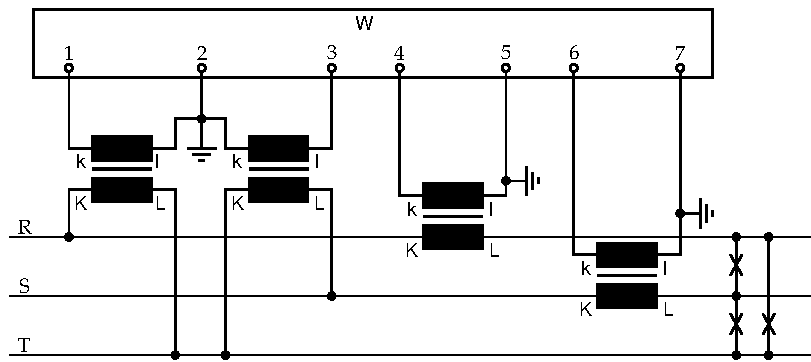
\includegraphics{Imatges/Cap-TrafosMesProt-Watt.pdf}
\end{figure}

A continuaci\'{o} es representa una insta{\l.l}aci\'{o} existent, amb dos TT i
dos TI, que alimenten a dos volt\'{\i}metres i a dos amper\'{\i}metres
respectivament; les c\`{a}rregues es troben a la dreta del circuit
primari. Es tracta d'afegir el nou watt\'{\i}metre a aquesta
insta{\l.l}aci\'{o}.

\begin{figure}[h]
\centering
    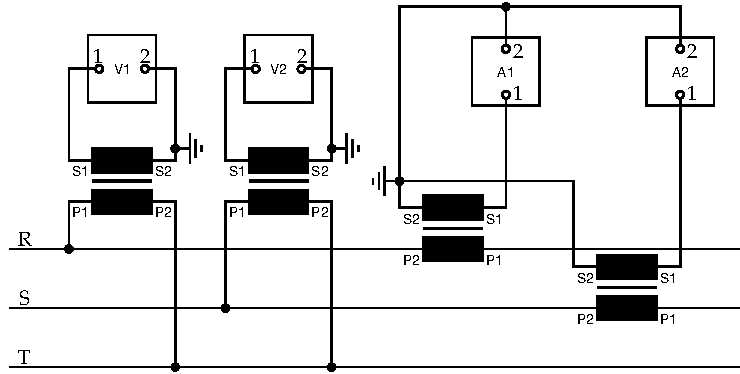
\includegraphics{Imatges/Cap-TrafosMesProt-Instal.pdf}
\end{figure}

Comencem fixant-nos en les tensions del watt\'{\i}metre, i veiem que cal
connectar-li la tensi\'{o} de la fase R al terminal 1, la tensi\'{o} de la
fase S al terminal 3, i la tensi\'{o} de la fase T al terminal 2.

Per aconseguir-ho en la nostra insta{\l.l}aci\'{o}, sense tocar el
connexionat dels dos volt\'{\i}metres existents, tan sols cal connectar
el terminal S1 del primer TT al terminal 1 del watt\'{\i}metre (tensi\'{o} de
la fase R), el terminal S1 del segon TT al terminal 3 del watt\'{\i}metre
(tensi\'{o} de la fase S), i el terminal S2 d'un qualsevol dels dos TT
al terminal 2 del watt\'{\i}metre (tensi\'{o} de la fase T).

Ens fixem a continuaci\'{o} en els corrents del watt\'{\i}metre. Si suposem
de forma arbitr\`{a}ria, uns corrents pels circuits primaris dels TI,
que vagin d'esquerra a dreta (aix\`{o} \'{e}s, cap a les c\`{a}rregues), veiem
que aquests corrents entren pels terminals K dels primaris dels TI,
i per tant surten, transformats, pels terminals k dels secundaris
dels TI. Aix\'{\i} doncs, el corrent que circula pel secundari del primer
TI, entra al watt\'{\i}metre pel terminal 4, i en surt pel terminal 5, i
el corrent que circula pel secundari del segon TI, entra al
watt\'{\i}metre pel terminal 6, i en surt pel terminal 7. Aquest sentit
de circulaci\'{o} dels corrents \'{e}s el que hem de mantenir, quan
connectem el watt\'{\i}metre a la nostra insta{\l.l}aci\'{o}.

Per aconseguir-ho en la nostra insta{\l.l}aci\'{o}, sense tocar el
connexionat dels dos amper\'{\i}metres existents, comencem per suposar un
sentit dels corrents primaris id\`{e}ntic al suposat anteriorment, \'{e}s a
dir cap a les c\`{a}rregues (aix\`{o} \'{e}s, d'esquerra a dreta). L'objectiu
ser\`{a} veure el sentit de circulaci\'{o} dels corrents de secundari
respecte dels terminals S1 dels dos TI, ja que disposem d'un fil per
a cadascun dels dos terminals de forma separada; no passa el mateix
amb els dos terminals S2, ja que \'{u}nicament disposem d'un fil pel
qual circula la suma dels dos corrents. Per tant, veiem que amb el
sentit de circulaci\'{o} que hem adoptat, aquests corrents surten pels
terminals P1 dels primaris dels TI, i per tant entren, transformats,
pels terminals S1 dels secundaris dels TI.

Aquests corrents que entren pels terminals S1, i que hem de dur al
watt\'{\i}metre, seran corrents que vistos des del watt\'{\i}metre, en
sortiran; per tant si ens fixem en l'an\`{a}lisi que hem fet en el
circuit inicial del watt\'{\i}metre, veiem que els terminal per on surten
els corrents s\'{o}n el 5 i el 7. Per tant ara queda clar que hem de
connectar el terminal S1 del primer TI, despr\'{e}s de passar per
l'amper\'{\i}metre \textsf{A1}, al terminal 5 del watt\'{\i}metre, i el
terminal S1 del segon TI, despr\'{e}s de passar per l'amper\'{\i}metre
\textsf{A2}, al terminal 7 del watt\'{\i}metre. Finalment, nom\'{e}s ens cal
tancar el circuit dels corrents secundaris, unint entre s\'{\i} els dos
terminals d'entrada 4  i 6, i connectant-los amb el fil com\'{u} que
uneix els dos terminals S2 dels dos TI.

Com es pot veure, no t\'{e} cap incid\`{e}ncia sobre el connexionat, quin \'{e}s
el terminal del secundari que est\`{a} connectat a terra, ni en el cas
dels TT ni en el cas dels TI.

A continuaci\'{o} es pot veure el connexionat complet, amb els dos
volt\'{\i}metres, els dos amper\'{\i}metres i el watt\'{\i}metre.

\begin{figure}[h]
\centering
    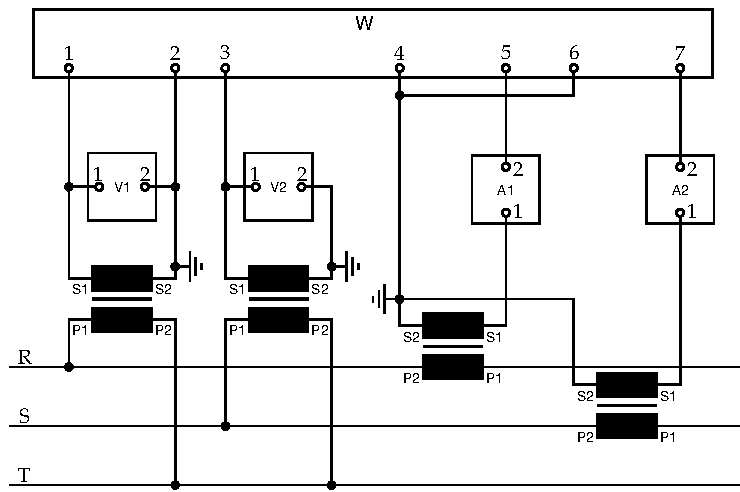
\includegraphics{Imatges/Cap-TrafosMesProt-Instal-Watt.pdf}
\end{figure}

\end{exemple}
